% Created 2024-02-13 ti 18:41
% Intended LaTeX compiler: pdflatex
\documentclass[12pt]{article}

%%%% settings when exporting code %%%% 

\usepackage{listings}
\lstdefinestyle{code-small}{
backgroundcolor=\color{white}, % background color for the code block
basicstyle=\ttfamily\small, % font used to display the code
commentstyle=\color[rgb]{0.5,0,0.5}, % color used to display comments in the code
keywordstyle=\color{black}, % color used to highlight certain words in the code
numberstyle=\ttfamily\tiny\color{gray}, % color used to display the line numbers
rulecolor=\color{black}, % color of the frame
stringstyle=\color[rgb]{0,.5,0},  % color used to display strings in the code
breakatwhitespace=false, % sets if automatic breaks should only happen at whitespace
breaklines=true, % sets automatic line breaking
columns=fullflexible,
frame=single, % adds a frame around the code (non,leftline,topline,bottomline,lines,single,shadowbox)
keepspaces=true, % % keeps spaces in text, useful for keeping indentation of code
literate={~}{$\sim$}{1}, % symbol properly display via latex
numbers=none, % where to put the line-numbers; possible values are (none, left, right)
numbersep=10pt, % how far the line-numbers are from the code
showspaces=false,
showstringspaces=false,
stepnumber=1, % the step between two line-numbers. If it's 1, each line will be numbered
tabsize=1,
xleftmargin=0cm,
emph={anova,apply,class,coef,colnames,colNames,colSums,dim,dcast,for,ggplot,head,if,ifelse,is.na,lapply,list.files,library,logLik,melt,plot,require,rowSums,sapply,setcolorder,setkey,str,summary,tapply},
aboveskip = \medskipamount, % define the space above displayed listings.
belowskip = \medskipamount, % define the space above displayed listings.
lineskip = 0pt} % specifies additional space between lines in listings
\lstset{style=code-small}
%%%% packages %%%%%

\usepackage[utf8]{inputenc}
\usepackage[T1]{fontenc}
\usepackage{lmodern}
\usepackage{textcomp}
\usepackage{color}
\usepackage{graphicx}
\usepackage{grffile}
\usepackage{wrapfig}
\usepackage{rotating}
\usepackage{longtable}
\usepackage{multirow}
\usepackage{multicol}
\usepackage{changes}
\usepackage{pdflscape}
\usepackage{geometry}
\usepackage[normalem]{ulem}
\usepackage{amssymb}
\usepackage{amsmath}
\usepackage{amsfonts}
\usepackage{dsfont}
\usepackage{array}
\usepackage{ifthen}
\usepackage{hyperref}
\usepackage{natbib}
\RequirePackage{setspace} % to modify the space between lines - incompatible with footnote in beamer
\renewcommand{\baselinestretch}{1.1}
\geometry{a4paper, left=10mm, right=10mm, top=10mm}
\usepackage{titlesec}
\usepackage{etoolbox}

\makeatletter
\patchcmd{\ttlh@hang}{\parindent\z@}{\parindent\z@\leavevmode}{}{}
\patchcmd{\ttlh@hang}{\noindent}{}{}{}
\makeatother
\RequirePackage{colortbl} % arrayrulecolor to mix colors
\definecolor{myorange}{rgb}{1,0.2,0}
\definecolor{mypurple}{rgb}{0.7,0,8}
\definecolor{mycyan}{rgb}{0,0.6,0.6}
\newcommand{\lightblue}{blue!50!white}
\newcommand{\darkblue}{blue!80!black}
\newcommand{\darkgreen}{green!50!black}
\newcommand{\darkred}{red!50!black}
\definecolor{gray}{gray}{0.5}
\hypersetup{
citecolor=[rgb]{0,0.5,0},
urlcolor=[rgb]{0,0,0.5},
linkcolor=[rgb]{0,0,0.5},
}
\newenvironment{note}{\small \color{gray}\fontfamily{lmtt}\selectfont}{\par}
\newenvironment{activity}{\color{orange}\fontfamily{qzc}\selectfont}{\par}
\RequirePackage{pifont}
\RequirePackage{relsize}
\newcommand{\Cross}{{\raisebox{-0.5ex}%
{\relsize{1.5}\ding{56}}}\hspace{1pt} }
\newcommand{\Valid}{{\raisebox{-0.5ex}%
{\relsize{1.5}\ding{52}}}\hspace{1pt} }
\newcommand{\CrossR}{ \textcolor{red}{\Cross} }
\newcommand{\ValidV}{ \textcolor{green}{\Valid} }
\usepackage{stackengine}
\usepackage{scalerel}
\newcommand\Warning[1][3ex]{%
\renewcommand\stacktype{L}%
\scaleto{\stackon[1.3pt]{\color{red}$\triangle$}{\tiny\bfseries !}}{#1}%
\xspace
}
\RequirePackage{fancyvrb}
\DefineVerbatimEnvironment{verbatim}{Verbatim}{fontsize=\small,formatcom = {\color[rgb]{0.5,0,0}}}
\definecolor{grayR}{HTML}{8A8990}
\definecolor{grayL}{HTML}{C4C7C9}
\definecolor{blueM}{HTML}{1F63B5}
\newcommand{\Rlogo}[1][0.07]{
\begin{tikzpicture}[scale=#1]
\shade [right color=grayR,left color=grayL,shading angle=60]
(-3.55,0.3) .. controls (-3.55,1.75)
and (-1.9,2.7) .. (0,2.7) .. controls (2.05,2.7)
and (3.5,1.6) .. (3.5,0.3) .. controls (3.5,-1.2)
and (1.55,-2) .. (0,-2) .. controls (-2.3,-2)
and (-3.55,-0.75) .. cycle;

\fill[white]
(-2.15,0.2) .. controls (-2.15,1.2)
and (-0.7,1.8) .. (0.5,1.8) .. controls (2.2,1.8)
and (3.1,1.2) .. (3.1,0.2) .. controls (3.1,-0.75)
and (2.4,-1.45) .. (0.5,-1.45) .. controls (-1.1,-1.45)
and (-2.15,-0.7) .. cycle;

\fill[blueM]
(1.75,1.25) -- (-0.65,1.25) -- (-0.65,-2.75) -- (0.55,-2.75) -- (0.55,-1.15) --
(0.95,-1.15)  .. controls (1.15,-1.15)
and (1.5,-1.9) .. (1.9,-2.75) -- (3.25,-2.75)  .. controls (2.2,-1)
and (2.5,-1.2) .. (1.8,-0.95) .. controls (2.6,-0.9)
and (2.85,-0.35) .. (2.85,0.2) .. controls (2.85,0.7)
and (2.5,1.2) .. cycle;

\fill[white]  (1.4,0.4) -- (0.55,0.4) -- (0.55,-0.3) -- (1.4,-0.3).. controls (1.75,-0.3)
and (1.75,0.4) .. cycle;

\end{tikzpicture}
}
\RequirePackage{epstopdf} % to be able to convert .eps to .pdf image files
\RequirePackage{capt-of} %
\RequirePackage{caption} % newlines in graphics
\RequirePackage{tikz-cd} % graph
\RequirePackage{booktabs} % for nice lines in table (e.g. toprule, bottomrule, midrule, cmidrule)
\RequirePackage{amsmath}
\RequirePackage{algorithm}
\RequirePackage[noend]{algpseudocode}
\RequirePackage{dsfont}
\RequirePackage{amsmath,stmaryrd,graphicx}
\RequirePackage{prodint} % product integral symbol (\PRODI)
\usepackage{ifthen}
\usepackage{xifthen}
\usepackage{xargs}
\usepackage{xspace}
\newcommand\defOperator[7]{%
\ifthenelse{\isempty{#2}}{
\ifthenelse{\isempty{#1}}{#7{#3}#4}{#7{#3}#4 \left#5 #1 \right#6}
}{
\ifthenelse{\isempty{#1}}{#7{#3}#4_{#2}}{#7{#3}#4_{#1}\left#5 #2 \right#6}
}
}
\newcommand\defUOperator[5]{%
\ifthenelse{\isempty{#1}}{
#5\left#3 #2 \right#4
}{
\ifthenelse{\isempty{#2}}{\underset{#1}{\operatornamewithlimits{#5}}}{
\underset{#1}{\operatornamewithlimits{#5}}\left#3 #2 \right#4}
}
}
\newcommand{\defBoldVar}[2]{
\ifthenelse{\equal{#2}{T}}{\boldsymbol{#1}}{\mathbf{#1}}
}
\newcommandx\Esp[2][1=,2=]{\defOperator{#1}{#2}{E}{}{\lbrack}{\rbrack}{\mathbb}}
\newcommandx\Prob[2][1=,2=]{\defOperator{#1}{#2}{P}{}{\lbrack}{\rbrack}{\mathbb}}
\newcommandx\Qrob[2][1=,2=]{\defOperator{#1}{#2}{Q}{}{\lbrack}{\rbrack}{\mathbb}}
\newcommandx\Var[2][1=,2=]{\defOperator{#1}{#2}{V}{ar}{\lbrack}{\rbrack}{\mathbb}}
\newcommandx\Cov[2][1=,2=]{\defOperator{#1}{#2}{C}{ov}{\lbrack}{\rbrack}{\mathbb}}
\newcommandx\Binom[2][1=,2=]{\defOperator{#1}{#2}{B}{}{(}{)}{\mathcal}}
\newcommandx\Gaus[2][1=,2=]{\defOperator{#1}{#2}{N}{}{(}{)}{\mathcal}}
\newcommandx\Wishart[2][1=,2=]{\defOperator{#1}{#2}{W}{ishart}{(}{)}{\mathcal}}
\newcommandx\Likelihood[2][1=,2=]{\defOperator{#1}{#2}{L}{}{(}{)}{\mathcal}}
\newcommandx\logLikelihood[2][1=,2=]{\defOperator{#1}{#2}{\ell}{}{(}{)}{}}
\newcommandx\Information[2][1=,2=]{\defOperator{#1}{#2}{I}{}{(}{)}{\mathcal}}
\newcommandx\Hessian[2][1=,2=]{\defOperator{#1}{#2}{H}{}{(}{)}{\mathcal}}
\newcommandx\Score[2][1=,2=]{\defOperator{#1}{#2}{S}{}{(}{)}{\mathcal}}
\newcommandx\Vois[2][1=,2=]{\defOperator{#1}{#2}{V}{}{(}{)}{\mathcal}}
\newcommandx\IF[2][1=,2=]{\defOperator{#1}{#2}{IF}{}{(}{)}{\mathcal}}
\newcommandx\Ind[1][1=]{\defOperator{}{#1}{1}{}{(}{)}{\mathds}}
\newcommandx\Max[2][1=,2=]{\defUOperator{#1}{#2}{(}{)}{min}}
\newcommandx\Min[2][1=,2=]{\defUOperator{#1}{#2}{(}{)}{max}}
\newcommandx\argMax[2][1=,2=]{\defUOperator{#1}{#2}{(}{)}{argmax}}
\newcommandx\argMin[2][1=,2=]{\defUOperator{#1}{#2}{(}{)}{argmin}}
\newcommandx\cvD[2][1=D,2=n \rightarrow \infty]{\xrightarrow[#2]{#1}}
\newcommandx\Hypothesis[2][1=,2=]{
\ifthenelse{\isempty{#1}}{
\mathcal{H}
}{
\ifthenelse{\isempty{#2}}{
\mathcal{H}_{#1}
}{
\mathcal{H}^{(#2)}_{#1}
}
}
}
\newcommandx\dpartial[4][1=,2=,3=,4=\partial]{
\ifthenelse{\isempty{#3}}{
\frac{#4 #1}{#4 #2}
}{
\left.\frac{#4 #1}{#4 #2}\right\rvert_{#3}
}
}
\newcommandx\dTpartial[3][1=,2=,3=]{\dpartial[#1][#2][#3][d]}
\newcommandx\ddpartial[3][1=,2=,3=]{
\ifthenelse{\isempty{#3}}{
\frac{\partial^{2} #1}{\partial #2^2}
}{
\frac{\partial^2 #1}{\partial #2\partial #3}
}
}
\newcommand\Real{\mathbb{R}}
\newcommand\Rational{\mathbb{Q}}
\newcommand\Natural{\mathbb{N}}
\newcommand\trans[1]{{#1}^\intercal}%\newcommand\trans[1]{{\vphantom{#1}}^\top{#1}}
\newcommand{\independent}{\mathrel{\text{\scalebox{1.5}{$\perp\mkern-10mu\perp$}}}}
\newcommand\half{\frac{1}{2}}
\newcommand\normMax[1]{\left|\left|#1\right|\right|_{max}}
\newcommand\normTwo[1]{\left|\left|#1\right|\right|_{2}}
\newcommand\Veta{\boldsymbol{\eta}}
\newcommand{\Model}{\mathcal{M}}
\newcommand{\ModelHat}{\widehat{\mathcal{M}}}
\newcommand{\param}{\Theta}
\newcommand{\paramHat}{\widehat{\param}}
\newcommand{\paramCon}{\widetilde{\param}}
\newcommand{\Vparam}{\boldsymbol{\param}}
\newcommand{\VparamT}{\Vparam_0}
\newcommand{\VparamHat}{\boldsymbol{\paramHat}}
\newcommand{\VparamCon}{\boldsymbol{\paramCon}}
\newcommand{\X}{X}
\newcommand{\x}{x}
\newcommand{\VZ}{\boldsymbol{Z}}
\newcommand{\VX}{\boldsymbol{X}}
\newcommand{\Vx}{\boldsymbol{x}}
\newcommand{\Y}{Y}
\newcommand{\y}{y}
\newcommand{\VY}{\boldsymbol{Y}}
\newcommand{\Vy}{\boldsymbol{y}}
\newcommand{\Vvarepsilon}{\boldsymbol{\varepsilon}}
\author{Brice Ozenne}
\date{\today}
\title{Overview of the package LMMstar}
\hypersetup{
 colorlinks=true,
 pdfauthor={Brice Ozenne},
 pdftitle={Overview of the package LMMstar},
 pdfkeywords={},
 pdfsubject={},
 pdfcreator={Emacs 27.2 (Org mode 9.5.2)},
 pdflang={English}
 }
\begin{document}

\maketitle
This vignette details how partial residuals can be used to illustrate
model fit in a linear regression and a linear mixed model when using
the package LMMstar. We thus start by loading the package:
\lstset{language=r,label= ,caption= ,captionpos=b,numbers=none}
\begin{lstlisting}
library(LMMstar)
\end{lstlisting}


\section{Univariate linear regression}
\label{sec:org0a67e79}

To illustrate the use of partial residuals we will use the \texttt{state.x77}
dataset:
\lstset{language=r,label= ,caption= ,captionpos=b,numbers=none}
\begin{lstlisting}
df1 <- data.frame(lifeExp = state.x77[,4],
                  illiteracy = state.x77[,3],
                  income = state.x77[,2]/1000,
                  murder = state.x77[,5],
                  edu = cut(state.x77[,6],c(0,50,60,100)))
head(df1,4)
\end{lstlisting}

\begin{verbatim}
         lifeExp illiteracy income murder      edu
Alabama    69.05        2.1  3.624   15.1   (0,50]
Alaska     69.31        1.5  6.315   11.3 (60,100]
Arizona    70.55        1.8  4.530    7.8  (50,60]
Arkansas   70.66        1.9  3.378   10.1   (0,50]
\end{verbatim}


 which contains information about life expectancy (\texttt{lifeExp}), income
(\texttt{income}), illeteracy (\texttt{illiteracy}), murder rate (\texttt{murder}), and the
percentage of high-school graduates (as categorical variable) in
various states in the USA. For later use we display a few descriptive
for each covariate value:
\lstset{language=r,label= ,caption= ,captionpos=b,numbers=none}
\begin{lstlisting}
summarize(lifeExp + illiteracy + income + murder + edu ~ 1, data = df1,
          columns = c("observed","missing","mean","min","max","sd"))
\end{lstlisting}

\begin{verbatim}
       outcome observed missing    mean    min    max        sd
1      lifeExp       50       0 70.8786 67.960 73.600 1.3423936
2   illiteracy       50       0  1.1700  0.500  2.800 0.6095331
3       income       50       0  4.4358  3.098  6.315 0.6144699
4       murder       50       0  7.3780  1.400 15.100 3.6915397
5  edu:(50,60]       50       0  0.5600  0.000  1.000 0.5014265
6 edu:(60,100]       50       0  0.1600  0.000  1.000 0.3703280
\end{verbatim}


and check there are no missing values. Here for the categorical
covariates the mean indicates the relative frequency of occurrence
(56\% and 16\%) and other columns like \texttt{sd} should be ignored.

\subsection{No interaction}
\label{sec:orgc75f255}

Suppose we are interested in relating life expectancy (\(Y\)) to
income (\(X\)). We cannot directly illustrate this relationship, as it
could be confounded by other variables such as illiteracy (\(Z_1\)),
murder rate (\(Z_2\)). and education (\(Z_3\)). We will therefore use
a linear model to control for those variables (\(\VZ=(Z_1,Z_2,Z_3)\))
where, for simplicity, we assume a linear effect for all variables:
\begin{align*}
Y = \alpha + \beta X + \gamma_1 Z_1 + \gamma_2 Z_2 + \gamma_2 Z_3 + \varepsilon
\end{align*}
\lstset{language=r,label= ,caption= ,captionpos=b,numbers=none}
\begin{lstlisting}
e.lm <- lmm(lifeExp ~ income + illiteracy + murder + edu, data = df1)
model.tables(e.lm)
\end{lstlisting}

\begin{verbatim}
              estimate         se      df      lower      upper      p.value
(Intercept) 71.5782755 1.13848841 44.0088 69.2838158 73.8727352 0.000000e+00
income       0.1926977 0.25264925 44.0088 -0.3164805  0.7018759 4.497063e-01
illiteracy   0.1759019 0.32096701 44.0088 -0.4709610  0.8227647 5.864356e-01
murder      -0.2782232 0.04785536 44.0088 -0.3746688 -0.1817776 6.328010e-07
edu(50,60]   0.3014130 0.41401530 44.0088 -0.5329753  1.1358013 4.704551e-01
edu(60,100]  0.7730650 0.51311796 44.0088 -0.2610505  1.8071804 1.390575e-01
\end{verbatim}


Note that the estimates are nearly identical to the ones of the \texttt{lm}
function:
\lstset{language=r,label= ,caption= ,captionpos=b,numbers=none}
\begin{lstlisting}
coef(e.lm) - coef(lm(lifeExp ~ income + illiteracy + murder + edu, data = df1))
\end{lstlisting}

\begin{verbatim}
  (Intercept)        income    illiteracy        murder    edu(50,60]   edu(60,100] 
-2.700062e-13  2.033929e-13 -2.898792e-13  6.272760e-15 -4.223843e-13 -5.306866e-13
\end{verbatim}


A graphical display can now be obtained by modifying the original
outcome, life expectancy, had every state had the same Illiteracy and
Murder:
\lstset{language=r,label= ,caption= ,captionpos=b,numbers=none}
\begin{lstlisting}
df1$pres <- residuals(e.lm, type = "partial", var = c("(Intercept)","income"))
head(df1)
\end{lstlisting}

\begin{verbatim}
           lifeExp illiteracy income murder      edu     pres
Alabama      69.05        2.1  3.624   15.1   (0,50] 72.88178
Alaska       69.31        1.5  6.315   11.3 (60,100] 71.41700
Arizona      70.55        1.8  4.530    7.8  (50,60] 72.10210
Arkansas     70.66        1.9  3.378   10.1   (0,50] 73.13584
California   71.71        1.1  5.114   10.3 (60,100] 73.60914
Colorado     72.06        0.7  4.884    6.8 (60,100] 73.05572
\end{verbatim}


By default, the partial residuals are computed substracting the effect
of the covariates, i.e. had each state got no illiteracy, no murder,
and the lowest education level:
\lstset{language=r,label= ,caption= ,captionpos=b,numbers=none}
\begin{lstlisting}
c(69.05 - 0.17590 * 2.1 - (-0.27822) * 15.1,
  69.31 - 0.17590 * 1.5 - (-0.27822) * 11.3 - 0.77306)
\end{lstlisting}

\begin{verbatim}
[1] 72.88173 71.41698
\end{verbatim}


This is why the element \texttt{"(Intercept)"} is specified in the \texttt{var}
argument: to avoid to substract the mean value from the outcome and
keep a plausible range of values for the outcome.

\bigskip

One may wish to compute the life expectancy had every state got a
specific illiteracy, murder rate, and education. Say the most common
in the sample: 1.17, 7.378, and (50,60] based on the descriptive
statistics. This can be obtained by specifying an attribute to the
argument type:
\lstset{language=r,label= ,caption= ,captionpos=b,numbers=none}
\begin{lstlisting}
type <- "partial"
attr(type, "reference") <- data.frame(illiteracy = 1.17, murder = 7.378,
                                      edu = factor("(50,60]",levels(df1$edu)))
df1$pres2 <- residuals(e.lm, type = type, var = c("(Intercept)","income"))
head(df1)
\end{lstlisting}

\begin{verbatim}
           lifeExp illiteracy income murder      edu     pres    pres2
Alabama      69.05        2.1  3.624   15.1   (0,50] 72.88178 71.33626
Alaska       69.31        1.5  6.315   11.3 (60,100] 71.41700 69.87149
Arizona      70.55        1.8  4.530    7.8  (50,60] 72.10210 70.55659
Arkansas     70.66        1.9  3.378   10.1   (0,50] 73.13584 71.59033
California   71.71        1.1  5.114   10.3 (60,100] 73.60914 72.06363
Colorado     72.06        0.7  4.884    6.8 (60,100] 73.05572 71.51021
\end{verbatim}


or computing by hand accounting for the reference level:
\lstset{language=r,label= ,caption= ,captionpos=b,numbers=none}
\begin{lstlisting}
c(69.05 - 0.17590 * (2.1-1.170) - (-0.27822) * (15.1-7.378) + 0.30141,
  69.31 - 0.17590 * (1.5-1.170) - (-0.27822) * (11.3-7.378) + 0.30141 - 0.77306)
\end{lstlisting}

\begin{verbatim}
[1] 71.33624 69.87148
\end{verbatim}


Note that changing the reference level only shift the partial residual
value by a constant, here:
\lstset{language=r,label= ,caption= ,captionpos=b,numbers=none}
\begin{lstlisting}
unique(df1$pres2 - df1$pres)
\end{lstlisting}

\begin{verbatim}
[1] -1.545513
\end{verbatim}


so does not affect the relation between the outcome (here \texttt{LifeExp})
and the exposure of interest (here \texttt{Income}). One can then get a
graphical display either manually using ggplot:
\lstset{language=r,label= ,caption= ,captionpos=b,numbers=none}
\begin{lstlisting}
gg.pres <- ggplot(df1) + geom_point(aes(x=income, y=pres))
gg.pres <- gg.pres + geom_abline(intercept = coef(e.lm)["(Intercept)"],
                                 slope = coef(e.lm)["income"])
gg.pres <- gg.pres + ggtitle("(B) partial residuals")
gg.pres
\end{lstlisting}

or directly via the plot function:
\lstset{language=r,label= ,caption= ,captionpos=b,numbers=none}
\begin{lstlisting}
plot(e.lm, time = "income", type = "partial", var = c("(Intercept)","income")) # C
plot(e.lm, time = "income", type = type, var = c("(Intercept)","income")) # D
\end{lstlisting}

\clearpage

These can be compared to displaying the observed outcome vs. income:
\lstset{language=r,label= ,caption= ,captionpos=b,numbers=none}
\begin{lstlisting}
gg.obs <- ggplot(df1) + geom_point(aes(x=income, y=lifeExp))
gg.obs <- gg.obs + ggtitle("(A) observed")
gg.obs
\end{lstlisting}

where it is apparent that by using the partial residuals, the data has
been normalized and exhibit less variability.
\begin{center}
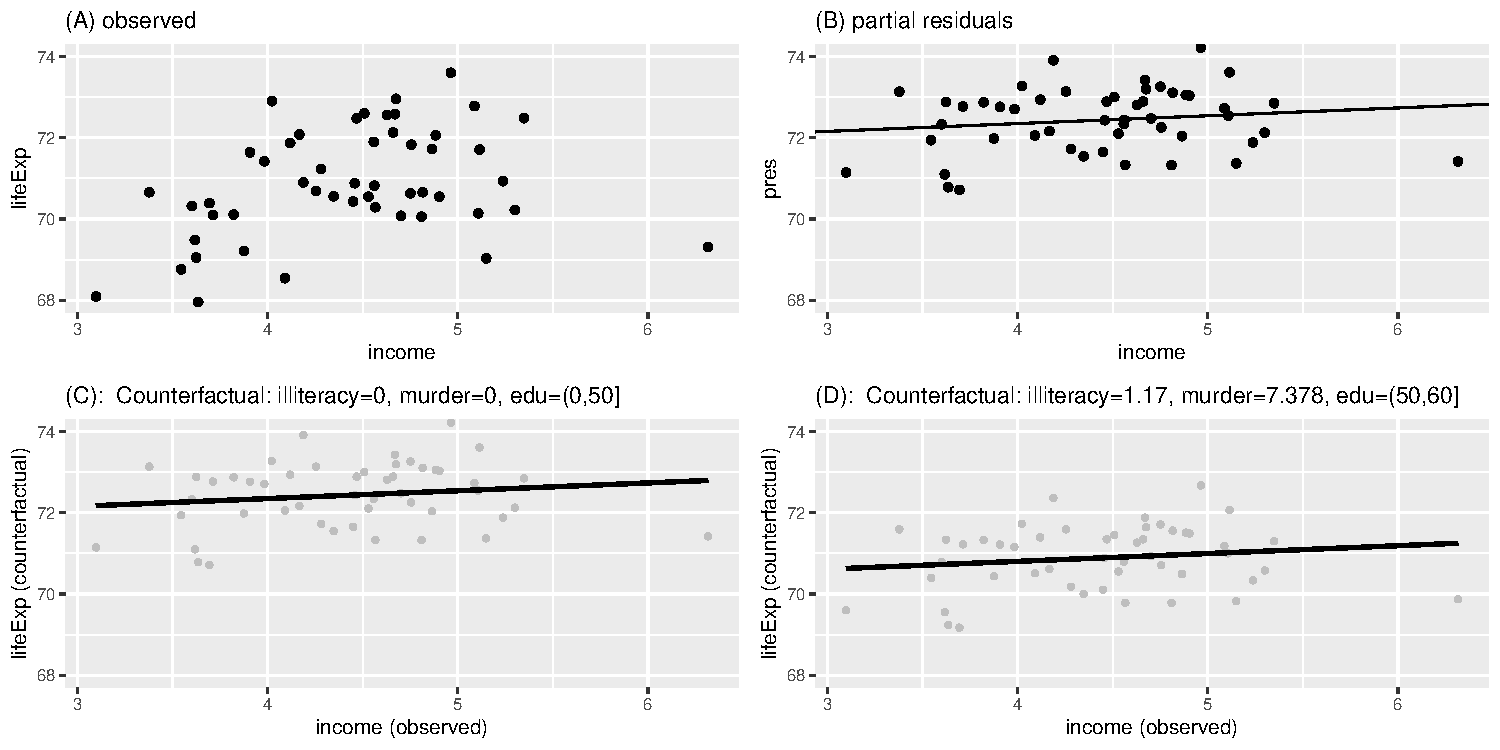
\includegraphics[trim={0 0 0 0},width=1\textwidth]{./figures/gg-lmpres-comparisons.pdf}
\end{center}

The output of the \texttt{plot} method is a list containing an element plot
with the ggplot object and an element data with the dataset. To avoid
actually displaying the graph one can use \texttt{autoplot} to only output the result:
\lstset{language=r,label= ,caption= ,captionpos=b,numbers=none}
\begin{lstlisting}
ls.plot <- autoplot(e.lm, time = "income", type = "partial", var = c("(Intercept)","income"))
str(ls.plot$data)
class(ls.plot$plot)
\end{lstlisting}

\begin{verbatim}
Classes 'residuals_lmm' and 'data.frame':	50 obs. of  3 variables:
 $ income   : num  3.62 6.32 4.53 3.38 5.11 ...
 $ fitted   : num  72.3 72.8 72.5 72.2 72.6 ...
 $ r.partial: num  72.9 71.4 72.1 73.1 73.6 ...
[1] "gg"     "ggplot"
\end{verbatim}


One can re-create the plot based on the data argument or modify the
existing plot based on the ggplot object, e.g. display with the y axis
between 68 and 74:
\lstset{language=r,label= ,caption= ,captionpos=b,numbers=none}
\begin{lstlisting}
ls.plot$plot  + coord_cartesian(ylim=c(68,74))
\end{lstlisting}

\bigskip

\subsection{What about confidence intervals?}
\label{sec:org84e5850}

A common question is whether one can display confidence intervals for
the regression line. It is possible to add confidence intervals on the
plot either via the argument \texttt{ci.alpha}:
\lstset{language=r,label= ,caption= ,captionpos=b,numbers=none}
\begin{lstlisting}
plot(e.lm, time = "income", type = "partial", var = c("(Intercept)","income"),
     ci.alpha = 0.25)
\end{lstlisting}

or by requesting confidence intervals for the fitted lines via the
argument \texttt{pres.ci} when calling \texttt{residuals}:
\lstset{language=r,label= ,caption= ,captionpos=b,numbers=none}
\begin{lstlisting}
pres.ci <- residuals(e.lm, type = "partial", var = c("(Intercept)","income"),
                     keep.data = TRUE, fitted.ci = TRUE)
head(pres.ci)
\end{lstlisting}

\begin{verbatim}
  lifeExp illiteracy income murder    edu   fitted fitted.lower fitted.upper r.partial
1   69.05          0  3.624      0 (0,50] 72.27661     71.11458     73.43864  72.88178
2   69.31          0  6.315      0 (0,50] 72.79516     71.10708     74.48324  71.41700
3   70.55          0  4.530      0 (0,50] 72.45120     71.25294     73.64945  72.10210
4   70.66          0  3.378      0 (0,50] 72.22921     71.04575     73.41266  73.13584
5   71.71          0  5.114      0 (0,50] 72.56373     71.25357     73.87389  73.60914
6   72.06          0  4.884      0 (0,50] 72.51941     71.26050     73.77832  73.05572
\end{verbatim}


which can be added to the previous graphical display, e.g.:
\lstset{language=r,label= ,caption= ,captionpos=b,numbers=none}
\begin{lstlisting}
gg.pres + geom_ribbon(data = pres.ci, alpha = 0.1,
                      aes(ymin = fitted.lower, ymax = fitted.upper, x = income))
\end{lstlisting}

The first plot is displayed in the left panel of the figure below. A
similar partial residual plot but now for the \texttt{murder} variable is
displayed in the right panel.

\begin{center}
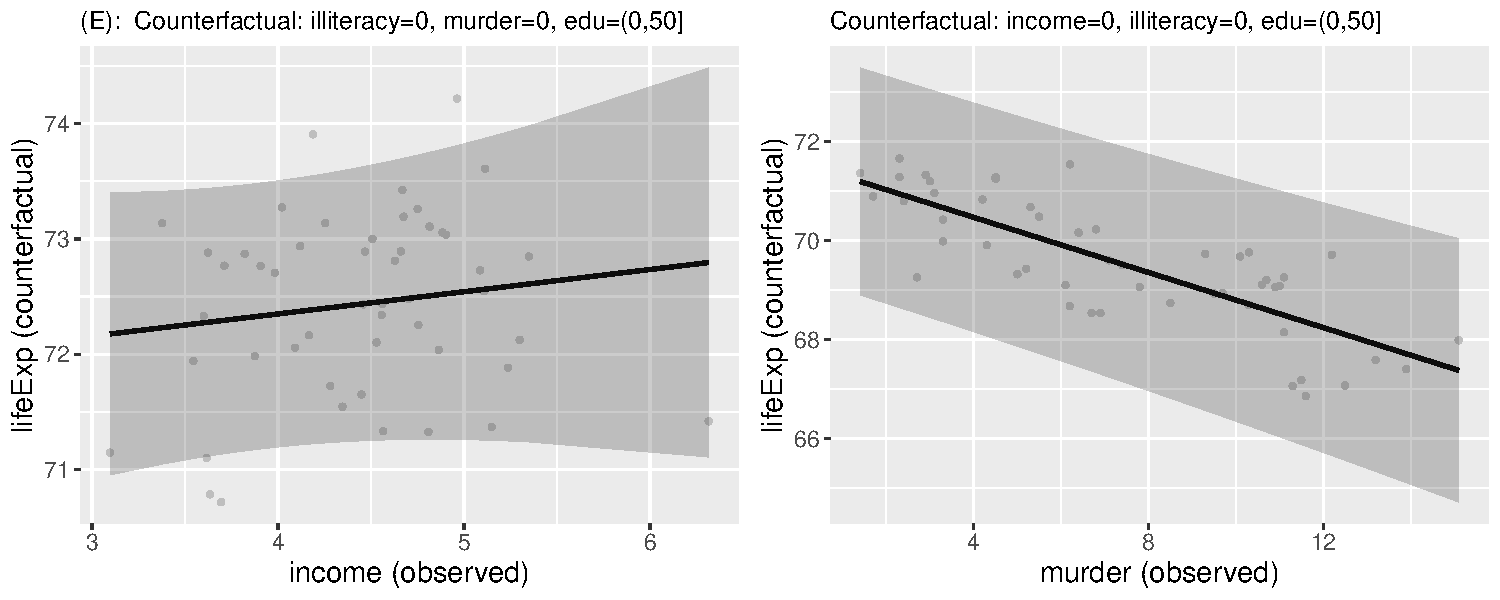
\includegraphics[trim={0 0 0 0},width=1\textwidth]{./figures/gg-lmpres-cifit.pdf}
\end{center}

In many case the uncertainty represented here is of little interest,
since it is the uncertainty of the intercept plus the exposure
effect. This is why even though the \texttt{murder} variable was highly
significant (p<0.001) whereas the income variable was not significant
(p=0.45) the confidence intervals looks large in both cases. To only
capture the uncertainty relative to the \texttt{income} or \texttt{murder} variable
one should remove the intercept value, e.g. by omitting
\texttt{"(Intercept)"} from the \texttt{var} argument:
\lstset{language=r,label= ,caption= ,captionpos=b,numbers=none}
\begin{lstlisting}
plot(e.lm, time = "income", type = "partial", var = "income", ci.alpha = 0.25)
plot(e.lm, time = "murder", type = "partial", var = "murder", ci.alpha = 0.25)
\end{lstlisting}
\begin{center}
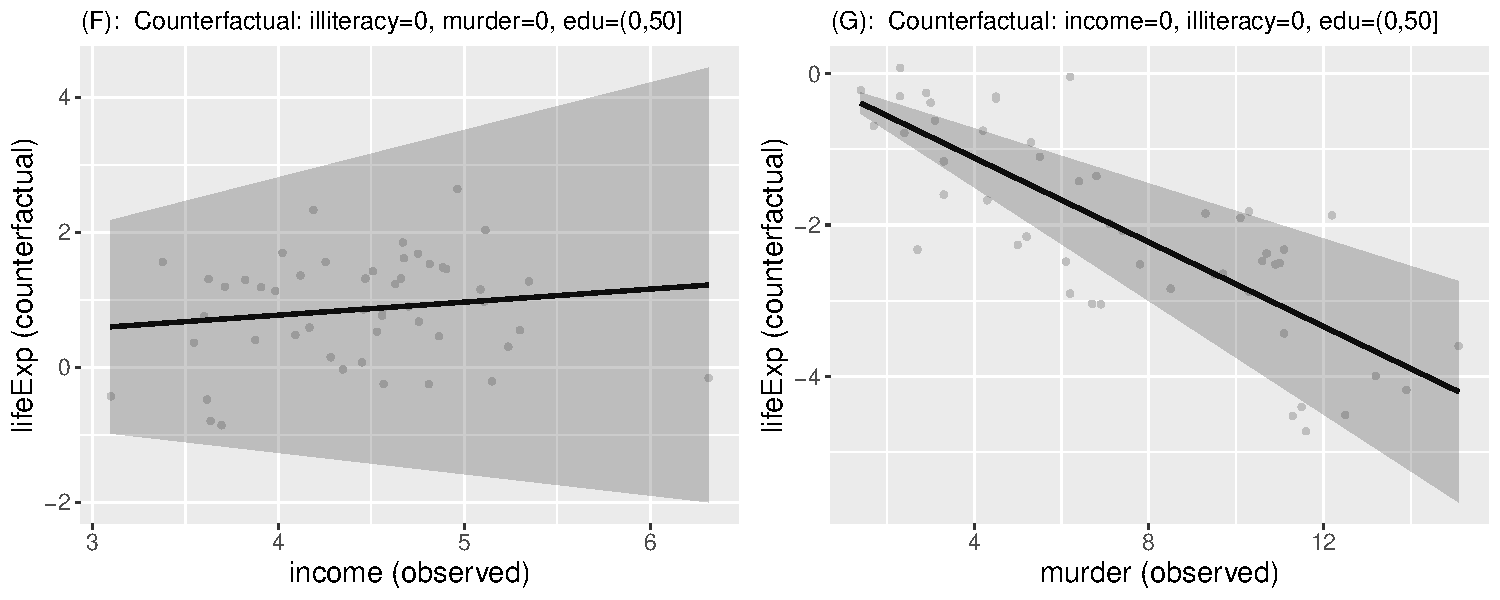
\includegraphics[trim={0 0 0 0},width=1\textwidth]{./figures/gg-lmpres-cicov.pdf}
\end{center}

The unpleasant side effect is that the range of values on the y-axis
appears unrealistic now. The statistical uncertainty may therefore be
better communicated otherwise, e.g. reporting confidence intervals or
p-values related to the covariate effect and keeping the partial
residual plot free of confidence intervals.

\subsection{Interaction with a categorical variable}
\label{sec:org1f09117}

Suppose that we are now interested in relating life expectancy (\(Y\))
to both income (\(X_1\)) for various level of education (\(X_2 \in
\{a,b,c\}\)), adjusting for other variables such as illiteracy
(\(Z_1\)) and murder rate (\(Z_2\)). As before we assume a linear
effect for all variables:
\begin{align*}
Y = \alpha + \beta_{1a} X_1 \Ind[X_2=a] + \beta_{1b} X_1 \Ind[X_2=b] + \beta_{1c} X_1 \Ind[X_2=c] + \gamma_1 Z_1 + \gamma_2 Z_2 + \varepsilon
\end{align*}
where \(\Ind[x]\) denotes the indicator variable taking value 1 when
\(x\) is true and 0 otherwise. This model can be estimated with the
following R code
\lstset{language=r,label= ,caption= ,captionpos=b,numbers=none}
\begin{lstlisting}
e.lmI <- lmm(lifeExp ~ income:edu + illiteracy + murder, data = df1)
model.tables(e.lmI)
\end{lstlisting}

\begin{verbatim}
                     estimate         se      df      lower      upper      p.value
(Intercept)        71.7858373 1.20951681 44.0088 69.3482301 74.2234444 0.000000e+00
illiteracy          0.1286978 0.31914517 44.0088 -0.5144934  0.7718890 6.887110e-01
murder             -0.2794017 0.04820845 44.0088 -0.3765589 -0.1822445 6.727632e-07
income:edu(0,50]    0.1714686 0.29772543 44.0088 -0.4285542  0.7714914 5.675972e-01
income:edu(50,60]   0.2252558 0.25210982 44.0088 -0.2828353  0.7333469 3.764587e-01
income:edu(60,100]  0.3037682 0.23692879 44.0088 -0.1737277  0.7812641 2.065179e-01
\end{verbatim}


\uline{Note:} this model is the same as \texttt{lmm(lifeExp \textasciitilde{} income*edu +
illiteracy + murder, data = df1)} but uses a different parametrisation.

\bigskip

Similarly as before, we can use the \texttt{plot} function to display the
partial residuals with respect to both \texttt{income} and \texttt{edu}:
\lstset{language=r,label= ,caption= ,captionpos=b,numbers=none}
\begin{lstlisting}
plot(e.lmI, time = "income", type = "partial", var = c("(Intercept)","income","edu"))
\end{lstlisting}

which can be compared to a plot assuming no interaction:
\lstset{language=r,label= ,caption= ,captionpos=b,numbers=none}
\begin{lstlisting}
plot(e.lm, time = "income", type = "partial", var = c("(Intercept)","income","edu"))
\end{lstlisting}

\begin{center}
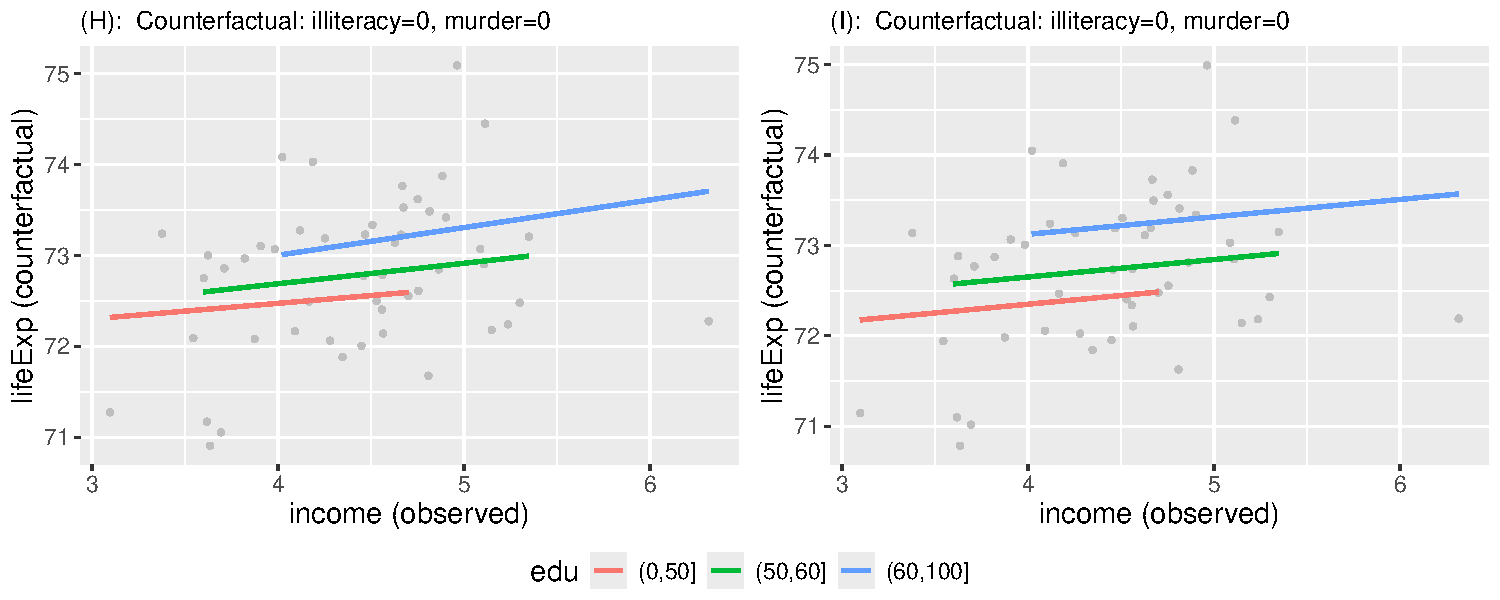
\includegraphics[trim={0 0 0 0},width=1\textwidth]{./figures/gg-lmpres-interaction.pdf}
\end{center}


The partial residuals can also be output via the \texttt{residuals} method:
\lstset{language=r,label= ,caption= ,captionpos=b,numbers=none}
\begin{lstlisting}
residuals(e.lmI, type = "partial", var = c("(Intercept)","income","edu"))[1:5]
\end{lstlisting}

\begin{verbatim}
[1] 72.99870 72.27419 72.49768 73.23743 74.44627
\end{verbatim}


and one can check that they are evaluated by substracting the effect
of the other variables (here \texttt{illiteracy} and \texttt{murder}), e.g.:
\lstset{language=r,label= ,caption= ,captionpos=b,numbers=none}
\begin{lstlisting}
c(69.05 - 0.12870 * 2.1 - (-0.27940) * 15.1,
  69.31 - 0.12870 * 1.5 - (-0.27940) * 11.3)
\end{lstlisting}

\begin{verbatim}
[1] 72.99867 72.27417
\end{verbatim}


Here we computed partial residuals representing the life expectancy in
the states had there be no murder nor illiteracy. We could also
consider the case of average murder rate and illiteracy. We would need
to define a new reference (i.e. drop \texttt{edu}):
\lstset{language=r,label= ,caption= ,captionpos=b,numbers=none}
\begin{lstlisting}
typeI <- "partial"
attr(typeI, "reference") <- data.frame(illiteracy = 1.17, murder = 7.378)
residuals(e.lmI, type = typeI, var = c("(Intercept)","income"))[1:5]
\end{lstlisting}

\begin{verbatim}
[1] 71.08785 70.36334 70.58683 71.32658 72.53542
\end{verbatim}


which we can also retrieve by hand:
\lstset{language=r,label= ,caption= ,captionpos=b,numbers=none}
\begin{lstlisting}
c(69.05 - 0.12870 * (2.1-1.170) - (-0.27940) * (15.1-7.378),
  69.31 - 0.12870 * (1.5-1.170) - (-0.27940) * (11.3-7.378))
\end{lstlisting}

\begin{verbatim}
[1] 71.08784 70.36334
\end{verbatim}



\clearpage

\section{Linear mixed model}
\label{sec:org6c35510}

To illustrate the use of partial residuals we will use data from a
two-arm randomized trial comparing the quality of the vision over time
of patients under placebo vs. active drug. We first re-shape the data:
\lstset{language=r,label= ,caption= ,captionpos=b,numbers=none}
\begin{lstlisting}
data(armd.wide, package = "nlmeU")
library(reshape2)
armd.long <- reshape2::melt(armd.wide,
                            measure.vars = paste0("visual",c(0,4,12,24,52)),
                            id.var = c("subject","lesion","treat.f","miss.pat"),
                            variable.name = "week",
                            value.name = "visual")
armd.long$week <- factor(armd.long$week, 
                         level = paste0("visual",c(0,4,12,24,52)),
                         labels = c(0,4,12,24,52))

\end{lstlisting}

make sure that 


\section{R session}
\label{sec:orgb8452f4}
Details of the R session used to generate this document:
\lstset{language=r,label= ,caption= ,captionpos=b,numbers=none}
\begin{lstlisting}
sessionInfo()
\end{lstlisting}

\begin{verbatim}
R version 4.2.0 (2022-04-22 ucrt)
Platform: x86_64-w64-mingw32/x64 (64-bit)
Running under: Windows 10 x64 (build 19045)

Matrix products: default

locale:
[1] LC_COLLATE=Danish_Denmark.utf8  LC_CTYPE=Danish_Denmark.utf8    LC_MONETARY=Danish_Denmark.utf8
[4] LC_NUMERIC=C                    LC_TIME=Danish_Denmark.utf8    

attached base packages:
[1] parallel  grid      stats     graphics  grDevices utils     datasets  methods   base     

other attached packages:
 [1] mice_3.14.0          sandwich_3.0-2       scales_1.2.1         rlang_1.1.1         
 [5] pbapply_1.7-0        numDeriv_2016.8-1.1  nlme_3.1-158         lava_1.7.2.1        
 [9] doSNOW_1.0.20        snow_0.4-4           iterators_1.0.14     foreach_1.5.2       
[13] copula_1.1-2         lme4_1.1-29          Matrix_1.5-1         LMMstar_1.0.0       
[17] ggpubr_0.4.0         multcomp_1.4-22      TH.data_1.1-1        MASS_7.3-57         
[21] survival_3.3-1       mvtnorm_1.2-3        qqtest_1.2.0         emmeans_1.8.8-090002
[25] ggplot2_3.4.3       

loaded via a namespace (and not attached):
 [1] butils.base_1.2     minqa_1.2.4         colorspace_2.1-0    ggsignif_0.6.3     
 [5] ellipsis_0.3.2      estimability_1.4.1  parameters_0.18.2   fs_1.6.3           
 [9] listenv_0.9.0       farver_2.1.1        remotes_2.4.2       gsl_2.1-8          
[13] fansi_1.0.4         codetools_0.2-18    splines_4.2.0       doParallel_1.0.17  
[17] cachem_1.0.8        pkgload_1.3.0       nloptr_2.0.3        broom_0.8.0        
[21] stabledist_0.7-1    effectsize_0.7.0.5  shiny_1.7.2         compiler_4.2.0     
[25] backports_1.4.1     fastmap_1.1.1       cli_3.6.1           later_1.3.0        
[29] htmltools_0.5.6     prettyunits_1.1.1   tools_4.2.0         lmerTest_3.1-3     
[33] coda_0.19-4         gtable_0.3.4        glue_1.6.2          reshape2_1.4.4     
[37] dplyr_1.1.3         Rcpp_1.0.11         carData_3.0-5       vctrs_0.6.3        
[41] insight_0.18.4      stringr_1.5.0       globals_0.16.2      ps_1.7.1           
[45] mime_0.12           miniUI_0.1.1.1      lifecycle_1.0.3     devtools_2.4.4     
[49] rstatix_0.7.0       future_1.31.0       zoo_1.8-11          promises_1.2.0.1   
[53] memoise_2.0.1       gridExtra_2.3       stringi_1.7.12      bayestestR_0.13.0  
[57] pcaPP_2.0-3         boot_1.3-28         pkgbuild_1.3.1      pkgconfig_2.0.3    
[61] lattice_0.20-45     purrr_1.0.2         htmlwidgets_1.6.2   labeling_0.4.3     
[65] cowplot_1.1.1       tidyselect_1.2.0    processx_3.6.1      parallelly_1.34.0  
[69] plyr_1.8.7          magrittr_2.0.3      R6_2.5.1            generics_0.1.3     
[73] profvis_0.3.7       ADGofTest_0.3       pillar_1.9.0        withr_2.5.1        
[77] mgcv_1.8-40         datawizard_0.6.1    abind_1.4-5         pspline_1.0-19     
[81] tibble_3.2.1        future.apply_1.10.0 crayon_1.5.1        car_3.1-0          
[85] utf8_1.2.3          urlchecker_1.0.1    usethis_2.1.6       data.table_1.14.2  
[89] callr_3.7.2         digest_0.6.33       xtable_1.8-4        tidyr_1.3.0        
[93] httpuv_1.6.5        stats4_4.2.0        munsell_0.5.0       sessioninfo_1.2.2
\end{verbatim}

\clearpage

\section*{References}
\label{sec:org9a9196a}
\begingroup
\renewcommand{\section}[2]{}

\bibliographystyle{apalike}
\bibliography{bibliography}

\endgroup

\clearpage

\appendix
\titleformat{\section}
{\normalfont\Large\bfseries}{Appendix~\thesection}{1em}{}

\renewcommand{\thefigure}{\Alph{figure}}
\renewcommand{\thetable}{\Alph{table}}
\renewcommand{\theequation}{\Alph{equation}}

\setcounter{figure}{0}    
\setcounter{table}{0}    
\setcounter{equation}{0}    
\end{document}